% =============================================================
%  Section: Theoretical framework
% =============================================================
\label{sec:theoretical_framework}

This section formalises the object-detection problem, presents the YOLOv1
grid formulation of \citet{redmon2016you}, derives the five-term loss
function used throughout this work, and defines the metrics employed in the
evaluation. The presentation follows the paper closely; we annotate the
points at which our COCO setting departs from the paper's VOC setting.

% -------------------------------------------------------------
\subsection{Object detection as a structured prediction problem}
\label{sec:theory:detection-problem}

A single-image object detector is a function
\[
  f_{\theta}\,:\,\mathbb{R}^{3 \times H \times W}\;\longrightarrow\;\bigl\{\,(c_i,\,b_i,\,s_i)\,\bigr\}_{i=1}^{n(x)}
\]
that takes an RGB image and produces a variable-length set of detections,
each consisting of a class label $c_i \in \{1,\,\ldots,\,C\}$, a bounding box
$b_i \in [0,1]^4$ in some agreed parameterisation, and a confidence score
$s_i \in [0,1]$. The number of detections $n(x)$ is itself a function of the
image, which distinguishes detection from classification (fixed output
length) and from semantic segmentation (one prediction per pixel).

Two algorithmic families have historically addressed this problem:

\begin{description}
    \item[Two-stage detectors.] R-CNN~\citep{girshick2014rich} and its
        successors Fast R-CNN~\citep{girshick2015fast} and
        Faster R-CNN~\citep{ren2015faster} first generate a candidate set of
        regions of interest (either via classical proposals such as selective
        search, or via a learnt region proposal network) and then classify
        each region independently. The decoupling of localisation and
        classification yields high precision but requires multiple forward
        passes per image.
    \item[Single-stage detectors.] YOLOv1~\citep{redmon2016you} and
        SSD~\citep{liu2016ssd} predict class and box jointly from a single
        forward pass of a convolutional network. Localisation accuracy is
        typically lower than in two-stage detectors, but inference is fast
        enough for real-time use.
\end{description}

\noindent YOLOv1 is the canonical single-stage detector and the subject of
this work. We summarise its core idea in the next subsection.

% -------------------------------------------------------------
\subsection{The YOLO grid formulation}
\label{sec:theory:grid}

YOLOv1 reformulates detection as a structured regression problem on a fixed
grid. The input image is divided into an $S \times S$ array of cells. Each
cell is responsible for detecting the objects whose centre falls within it.
For every cell the network outputs:
\begin{itemize}
    \item $B$ candidate bounding boxes, each parameterised by
        $(x,\,y,\,w,\,h,\,\text{conf})$, where $(x,y)$ is the centre of the
        box and $\text{conf}$ is the predicted IoU between this box and the
        ground-truth object that the cell is responsible for.
    \item A single set of $C$ class probabilities, shared across the $B$
        boxes (one set of class scores per cell, not per box).
\end{itemize}

\noindent The per-cell output therefore has $C + 5B$ channels, and the full
prediction tensor has shape $(S, S, C + 5B)$. For the VOC setting of the
original paper ($S = 7$, $B = 2$, $C = 20$) this comes to $S^2(C+5B) = 1\,470$
output values per image. For the COCO setting used throughout this work
($C = 80$) it grows to $4\,410$.

\paragraph{Coordinate parameterisation.} The centre coordinates $(x, y)$ of a
predicted box are expressed \emph{relative to the cell} that contains the
ground-truth centre, so they lie in $[0, 1]$ with $(0, 0)$ at the top-left
corner of the cell and $(1, 1)$ at the bottom-right. The width and height
$(w, h)$ are expressed \emph{relative to the whole image}, also in $[0, 1]$.
This asymmetry is deliberate: an object can straddle multiple cells, but its
centre falls in exactly one. Coordinates relative to the cell would force
$w, h$ to exceed $1$ for any non-tiny object, which would interact poorly
with the loss's $\sqrt{\cdot}$ transform. This is the same asymmetry that
caused Bug~2 in Section~\ref{sec:bug:wh-decoding}.

\paragraph{Per-cell tensor layout.} The $C + 5B$ channels at each grid cell
are arranged as
\[
  \underbrace{[\,p_1,\,\ldots,\,p_{C}\,]}_{\text{class probs}}\;
  \underbrace{[\,\text{conf}_1,\,x_1,\,y_1,\,w_1,\,h_1\,]}_{\text{box 1}}\;
  \underbrace{[\,\text{conf}_2,\,x_2,\,y_2,\,w_2,\,h_2\,]}_{\text{box 2}}\;\cdots
\]
with the second box's channels immediately following the first, and so on
for $B > 2$. The ground-truth tensor uses the same layout but populates only
the first box slot: there is one ground-truth box per cell, not~$B$ of them.
The second slot is structurally present in the target but left at zero, and
is read only by the predicted side during loss computation. This is the
specific layout that was misindexed in V1--V4 (cf.\ Section
\ref{sec:bug:loss-indices}).

\paragraph{The one-object-per-cell constraint.} At training time, if two
ground-truth box centres fall in the same cell, only one of them is kept; the
other is dropped. The detector therefore cannot, by construction, recover
both. This is a hard limitation of the YOLOv1 formulation and is one of the
primary failure modes observed in Section~\ref{sec:results:perclass}, where
classes that frequently co-occur in tight clusters (forks, knives and spoons
on dining tables; multiple sports balls in foreground photographs) register
particularly low AP.

% -------------------------------------------------------------
\subsection{The five-term loss}
\label{sec:theory:loss}

The training objective is a sum of squared errors over five terms,
implementing what \citet{redmon2016you} describe as a multi-task loss that
balances localisation, confidence and classification. The full expression is

\begin{align}
  \mathcal{L} \;=\;&
    \lambda_{\text{coord}} \!\!\sum_{i=0}^{S^2}\!\sum_{j=0}^{B}\!
      \mathbb{1}^{\text{obj}}_{ij}\Bigl[
        (x_i - \hat{x}_i)^2 + (y_i - \hat{y}_i)^2
      \Bigr] \notag\\[2pt]
  +\;&
    \lambda_{\text{coord}} \!\!\sum_{i=0}^{S^2}\!\sum_{j=0}^{B}\!
      \mathbb{1}^{\text{obj}}_{ij}\Bigl[
        \bigl(\sqrt{w_i} - \sqrt{\hat{w}_i}\bigr)^2 +
        \bigl(\sqrt{h_i} - \sqrt{\hat{h}_i}\bigr)^2
      \Bigr] \label{eq:loss}\\[2pt]
  +\;& \sum_{i=0}^{S^2}\!\sum_{j=0}^{B}\!
        \mathbb{1}^{\text{obj}}_{ij}\bigl(C_i - \hat{C}_i\bigr)^2 \notag\\[2pt]
  +\;& \lambda_{\text{noobj}}\!\!\sum_{i=0}^{S^2}\!\sum_{j=0}^{B}\!
        \mathbb{1}^{\text{noobj}}_{ij}\bigl(C_i - \hat{C}_i\bigr)^2 \notag\\[2pt]
  +\;& \sum_{i=0}^{S^2}\!
        \mathbb{1}^{\text{obj}}_{i}\!\!\sum_{c \in \text{classes}}\!\!
        \bigl(p_i(c) - \hat{p}_i(c)\bigr)^2 \notag
\end{align}

\noindent where hatted quantities are predictions and unhatted are ground
truth. The two indicator functions are defined as
\[
  \mathbb{1}^{\text{obj}}_{ij} =
    \begin{cases}
      1 & \text{if box $j$ in cell $i$ is responsible for an object,}\\
      0 & \text{otherwise,}
    \end{cases}
  \qquad
  \mathbb{1}^{\text{noobj}}_{ij} = 1 - \mathbb{1}^{\text{obj}}_{ij},
\]
with $\mathbb{1}^{\text{obj}}_{i}$ being the cell-level OR over the $B$ boxes
(it is $1$ iff cell $i$ contains a ground-truth centre). The five terms can
be read off the rows of Equation~\eqref{eq:loss}; an annotated diagrammatic
version is provided in Figure~\ref{fig:loss-explained}.

\begin{figure}[!ht]
\centering
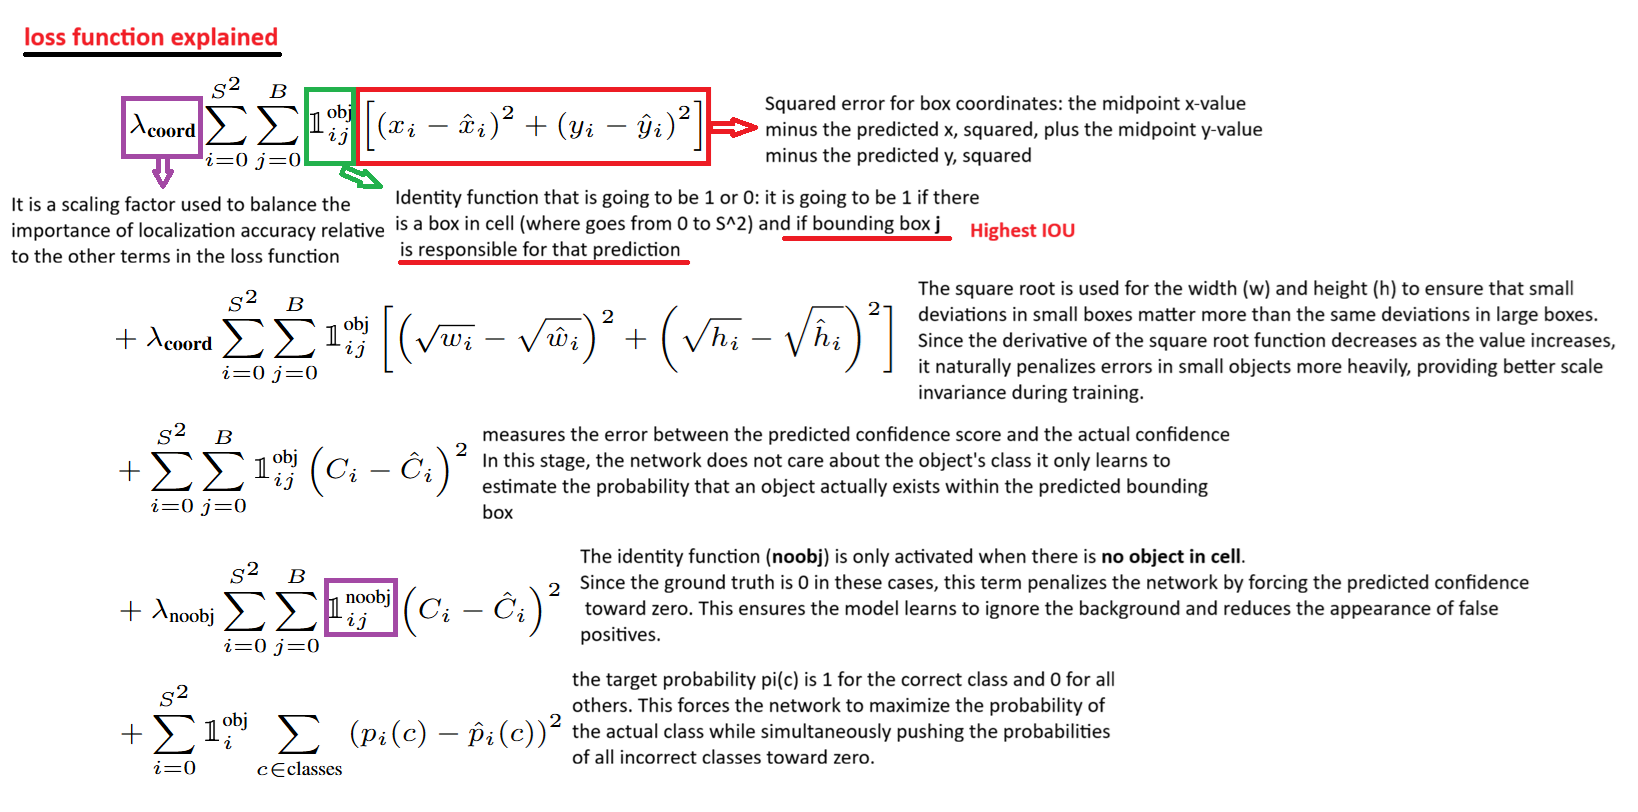
\includegraphics[width=0.95\textwidth]{loss_function_explained.png}
\caption{Annotated diagram of the YOLOv1 loss. The five terms are shown in
the original paper's notation, with handwritten annotations describing the
purpose of each summand. The figure is the author's own annotation of the
loss diagram in \citet{redmon2016you}.}
\label{fig:loss-explained}
\end{figure}

\paragraph{Term-by-term reading.}

\begin{enumerate}
    \item \emph{Centre-coordinate term.} Penalises the squared error in
        $(x, y)$ at cells with objects, summed only over the box that is
        responsible for the object. Weighted by $\lambda_{\text{coord}} = 5$
        so that localisation receives a larger gradient signal than
        classification, which has many more contributing summands.
    \item \emph{Size term.} Penalises the squared error in $\sqrt{w}$ and
        $\sqrt{h}$ rather than in $w$ and $h$ directly. The square root has
        the geometric effect of compressing the dynamic range of the box
        sizes: a $0.1$ error on a box of width $0.1$ is far more important
        than the same absolute error on a box of width $0.9$. Without the
        square root, large boxes would dominate the gradient and small
        objects would never be localised properly.
    \item \emph{Object-confidence term.} For each cell that contains an
        object, the confidence of the \emph{responsible} predictor is pulled
        towards the IoU between that predictor's box and the ground-truth
        box. The responsibility assignment uses the higher-IoU of the $B$
        candidate boxes per cell (see below).
    \item \emph{No-object confidence term.} For every box in every cell that
        does \emph{not} contain an object, the confidence is pulled towards
        zero. This term has by far the largest number of contributing
        summands; without the down-weighting by
        $\lambda_{\text{noobj}} = 0.5$ it would overwhelm the per-object
        signal and the model would converge to predicting confidence zero
        everywhere.
    \item \emph{Class term.} Pulls the predicted class distribution at each
        object-containing cell towards the one-hot ground-truth distribution.
        This term is computed once per cell (not per box), which is
        equivalent to saying that all $B$ boxes in a cell share the same
        class prediction.
\end{enumerate}

\paragraph{Responsibility.} The original paper assigns responsibility for an
object to the predicted box with the highest IoU against the ground-truth
box. At training time, for each cell that contains an object, the two
predicted boxes are evaluated against the single ground-truth box; the box
with the larger IoU is marked as responsible, and only its $(x, y, w, h,
\text{conf})$ tuple contributes to the centre, size and object-confidence
terms. The losing box contributes only through the no-object confidence term.
The intuition is that the two boxes per cell are not redundant: over
training, they specialise in different aspect ratios (one tall, one wide, for
example), with the responsibility assignment acting as a soft selector.

\paragraph{The $\sqrt{\cdot}$ pitfall.} The network output is unconstrained,
so a predicted $w$ or $h$ may be negative early in training. The square root
of a negative number is undefined for real-valued tensors; if the loss is
implemented naively as \texttt{torch.sqrt(w)}, the first negative prediction
produces a NaN that propagates through the rest of the batch. A robust
implementation uses $\operatorname{sign}(x) \cdot \sqrt{|x| + \varepsilon}$,
preserving the sign so that the gradient on the next step points back into
the positive half-line. This is the form used in \texttt{src/loss.py} and is
discussed in Section~\ref{sec:impl:loss}.

% -------------------------------------------------------------
\subsection{Intersection over Union}
\label{sec:theory:iou}

The Intersection-over-Union ratio (IoU, also called the Jaccard index) is the
fundamental geometric measure used throughout the loss and the evaluation
metric. For two axis-aligned bounding boxes $A$ and $B$, both expressed in
the same coordinate system, it is defined as
\[
  \mathrm{IoU}(A, B) \;=\; \frac{|A \cap B|}{|A \cup B|}
                     \;=\; \frac{|A \cap B|}{|A| + |B| - |A \cap B|},
\]
where $|\cdot|$ denotes box area. The ratio takes values in $[0, 1]$, with
$0$ for disjoint boxes and $1$ for identical boxes. In the loss, IoU is
computed between each of the $B$ predicted boxes and the single ground-truth
box per cell in order to assign responsibility. In the evaluation, IoU is
computed between every prediction and every ground-truth box of the same
class to decide whether the prediction is a true or false positive.

\paragraph{Implementation note.} For two boxes given in midpoint form
$(x_c, y_c, w, h)$ the intersection rectangle has corners
\[
  x_1 = \max\!\bigl(x_c^{A} - w^{A}/2,\;x_c^{B} - w^{B}/2\bigr), \quad
  x_2 = \min\!\bigl(x_c^{A} + w^{A}/2,\;x_c^{B} + w^{B}/2\bigr),
\]
and similarly for $y$. Its area is
$\max(0,\,x_2-x_1)\cdot\max(0,\,y_2-y_1)$; the clamp at zero handles the
no-overlap case, which would otherwise produce a negative ``area''. The
denominator adds a small $\varepsilon = 10^{-6}$ to avoid division by zero
when both boxes have zero area.

% -------------------------------------------------------------
\subsection{Mean Average Precision}
\label{sec:theory:map}

Mean Average Precision at IoU threshold $\tau$ (mAP@$\tau$) is the standard
detection metric introduced by the Pascal VOC
challenge~\citep{everingham2010pascal} and adopted by
COCO~\citep{lin2014microsoft}. It captures both how well the model localises
objects (via the IoU threshold) and how well it ranks them by confidence
(via the precision--recall integration).

\paragraph{Per-class Average Precision.} Fix a class $c$ and a test set with
$N_c$ ground-truth instances of that class across all images. The model
produces a list of predictions $\{(s_k, \mathrm{box}_k)\}_{k=1}^{M_c}$ for
class $c$, where $s_k$ is the predicted confidence. Sort the list by
decreasing confidence. Walk through it in that order, maintaining a count of
true positives (TP) and false positives (FP). A prediction is a true positive
if it has $\mathrm{IoU} \ge \tau$ against a ground-truth box \emph{that has
not yet been claimed} by an earlier (higher-confidence) prediction; otherwise
it is a false positive. Once a ground-truth box is claimed, subsequent
predictions overlapping it count as duplicates and are recorded as false
positives.

After step $k$ of the walk, the running precision and recall are
\[
  P_k = \frac{\mathrm{TP}_k}{\mathrm{TP}_k + \mathrm{FP}_k}, \qquad
  R_k = \frac{\mathrm{TP}_k}{N_c}.
\]
The Average Precision for class $c$ is the area under the precision--recall
curve, evaluated by trapezoidal integration with an additional anchor at
$(R, P) = (0, 1)$ to make the integration well-defined at the leftmost
endpoint:
\[
  \mathrm{AP}_c \;=\; \int_{0}^{1} P_c(R)\,\mathrm{d}R \;\approx\;
    \sum_{k=1}^{M_c} \frac{P_{k-1} + P_k}{2}\,\bigl(R_k - R_{k-1}\bigr).
\]
The mean Average Precision is then the mean of the per-class AP over the
$C$ classes:
\[
  \mathrm{mAP}@\tau \;=\; \frac{1}{C}\sum_{c=1}^{C} \mathrm{AP}_c(\tau).
\]
The original VOC challenge fixes $\tau = 0.5$; COCO additionally reports
mAP averaged over $\tau \in \{0.5, 0.55, \ldots, 0.95\}$, denoted
mAP@$[0.5\!:\!0.05\!:\!0.95]$. In this work we report only mAP@0.5, both
because it is the headline metric of \citet{redmon2016you} and because at
this level of absolute performance the 0.5 threshold already separates
classes meaningfully.

\paragraph{The claimed-GT bookkeeping.} The detail that distinguishes mAP
from a naive precision/recall computation is the rule that each ground-truth
instance can be claimed by at most one prediction. Two predictions that both
overlap the same ground-truth box at $\mathrm{IoU} \ge \tau$ count as one TP
and one FP rather than as two TPs; the FP is the duplicate. This is the
mechanism that penalises a model which hedges by emitting multiple
high-confidence predictions for the same object. In our implementation the
claimed status is tracked as a boolean vector per image and per class,
indexed by the position of the ground-truth box in the per-image GT list.

\paragraph{Skipping empty classes.} A class that has zero ground-truth
instances in the evaluated split has an undefined AP (division by zero in
the recall computation). The convention used in this work, and in most
public mAP implementations, is to drop such classes from the mean rather
than count them as AP~$=$~$0$. On COCO this never triggers because every
class is represented in the test split, but the rule matters when this same
code is repurposed for smaller benchmarks.

% -------------------------------------------------------------
\subsection{Backbones and transfer learning}
\label{sec:theory:backbone}

The detection-head equations above are agnostic to which convolutional
backbone produces the feature map fed to the dense layers. Two
choices are relevant to this work.

\begin{description}
    \item[Darknet24] is the custom 24-layer convolutional network proposed in
        \citet{redmon2016you}. It alternates $3\!\times\!3$ and
        $1\!\times\!1$ convolutions, uses LeakyReLU activations, and is
        pretrained on ImageNet by the paper's authors before the detection
        fine-tuning step. We reproduced this backbone for V1--V3 and trained
        it from scratch (i.e.\ without the ImageNet pretraining stage), with
        the consequences described in Sections~\ref{sec:experiments:v1}
        to~\ref{sec:experiments:v3}.
    \item[ResNet18] is the smallest member of the residual-network family of
        \citet{he2016deep}. Residual networks introduce identity shortcut
        connections that allow gradients to flow through deep stacks of
        convolutional layers without vanishing, and have become the default
        ImageNet-classification backbone in much of the field. PyTorch's
        \texttt{torchvision} package ships ResNet18 with a pretrained
        ImageNet checkpoint, which we use directly to bootstrap V4--V6.
\end{description}

\paragraph{Transfer learning.} The reason ImageNet pretraining matters is
that the features learnt to classify natural images at $224\!\times\!224$
resolution are also useful for localising those same objects at higher
resolutions. A randomly initialised convolutional network of comparable
depth, faced with the cold-start problem of learning low-level edges,
mid-level textures and high-level object parts simultaneously while also
learning the detection-specific head, typically requires substantially more
training data and steps than the same network initialised from an ImageNet
checkpoint. The V1--V3 runs trained from scratch on COCO illustrate the
practical cost of skipping this step. The V4 run, which switched to a
pretrained ResNet18, was the first that converged to a low validation loss
within the budget allocated, although as Section~\ref{sec:experiments:v4}
discusses, low validation loss turned out not to be sufficient given the
bugs that V4 still inherited.

\medskip

This concludes the theoretical preliminaries. The next section translates
each of these formal definitions into runnable PyTorch code.
